\section{Background and Previous Works}

This section will walk through the concept of transfer learning that we are using in this work. Secondly, the explanation for the model architecture will be provided. Lastly, we briefly talk about the hardware that we use to benchmark in this work.

\subsection{Transfer Learning}

Transfer Learning is a method of machine learning. You can use the pre-trained model from the large general dataset to train your dataset or target tasks with a smaller dataset size, which is more efficient than training the model from scratch.~\cite{brownlee2017gentle}

\subsection{Transformer, BERT, RoBERTa, and GPT-2}

The Transformer is a model architecture of deep learning. It works with stacked self-attention and encoder/decoder stacks.~\cite{vaswani2017attention}

Bidirectional Encoder Representations (or BERT) from Transformers is sophisticated modified version of encoder part from transformer-based language model. It can be used as a pre-trained model from a large corpus to fine-tune with the specific dataset.~\cite{devlin2018bert} For RoBERTa, it is a transformer-based language model with an optimized method from the BERT model. RoBERTa is built on BERT but has different key hyperparameters, implementation, trained with dynamic masking, and removal of BERT's next sentence.~\cite{liu2019roberta}

GPT-2 is also a transformer-based language model with 1.5 billion parameters. It trained by large dataset from internet with 8 million web pages. Since it is a bloated model, it can learn with zero-shot setting.~\cite{radford2019better}

\begin{figure}[htbp]
  \centering
  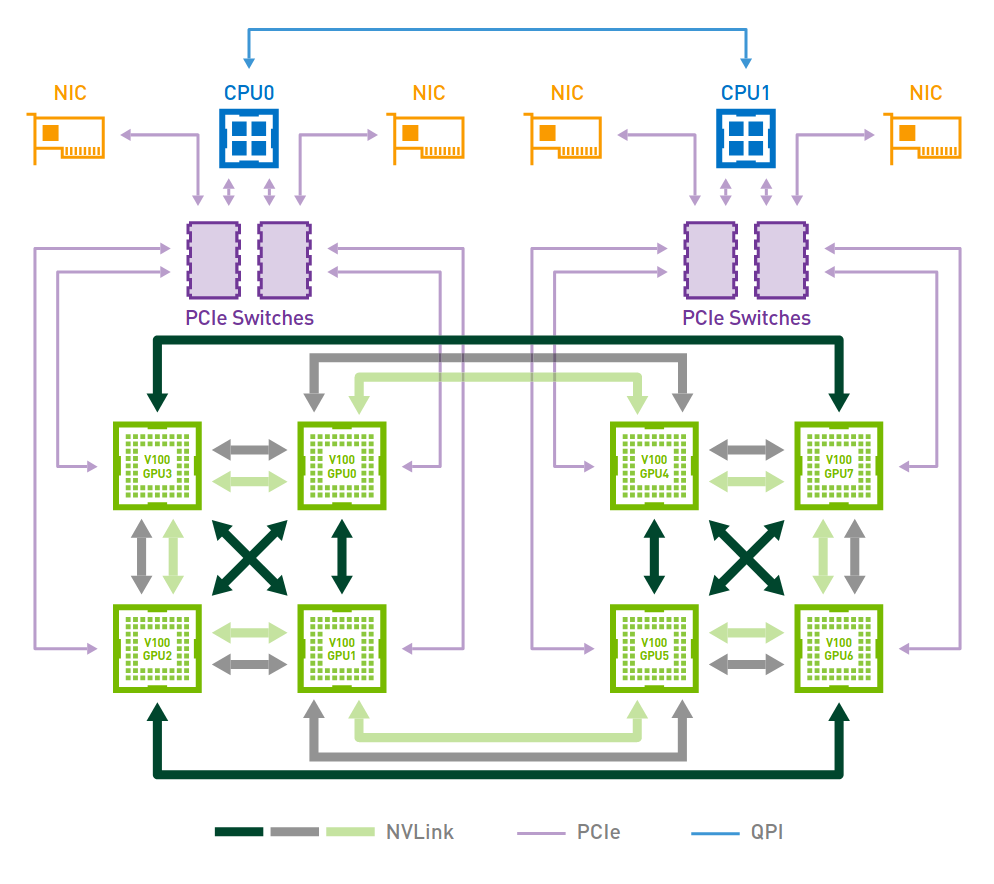
\includegraphics[width=0.6\linewidth]{fig/dgx-arch.png}
  \caption{Schematic view of DGX-1. Image taken from \cite{dgx-1}}
  \label{fig:dgx}
\end{figure}



\subsection{NVIDIA DGX-1}

The testing hardware is NVIDIA DGX-1. It consists of 8$\times$Tesla V100 GPUs, and each of them has 32 GB of attached memory. High level overview of this architecture is illustrated in Figure~\ref{fig:dgx}. The characteristic of these multi-GPUs devices is the NVLink. It is the inter-connection to reduce network latency in data sending across the devices. \cite{dgx-1}
